\documentclass[twocolumn,landscape,8pt]{article}
\usepackage{lipsum}% http://ctan.org/pkg/lipsum
\usepackage{graphicx,dblfloatfix}% http://ctan.org/pkg/{graphicx,dblfloatfix}
\usepackage{longtable}
\usepackage{tikz}
\usepackage{blindtext}
\usepackage{calendar} % Use the calendar.sty style
\usepackage[condensed,math]{anttor}
\usepackage[T1]{fontenc}
\usepackage{bchart}

\usepackage[landscape,margin=0.5in]{geometry}
\newcommand\framethispage[1][1cm]{%
    \tikz[overlay,remember picture,line width=1pt]
    \draw([xshift=(#1),yshift=(-#1)]current page.north west)rectangle
         ([xshift=(-#1),yshift=(#1)]current page.south east);%
}

\begin{document}
\framethispage[0.2cm]% le cadre est à 2 cm des bords de la feuille
\newcounter{a}
\newcounter{b}

%----------------------------------------------------------
\newcommand{\slice}[4]{
  \pgfmathparse{0.5*#1+0.5*#2}
  \let\midangle\pgfmathresult

   slice
  \draw[thick,fill=black!10] (0,0) -- (#1:1) arc (#1:#2:1) -- cycle;

   outer label
  \node[label=\midangle:#4] at (\midangle:1) {};

   inner label
  \pgfmathparse{min((#2-#1-10)/110*(-0.3),0)}
  \let\temp\pgfmathresult
  \pgfmathparse{max(\temp,-0.5) + 0.8}
  \let\innerpos\pgfmathresult
  \node at (\midangle:\innerpos) {#3};
}
%----------------------------------------------------------

\title{Finance}

Example de la police que je voulais
\makeatletter
\newcommand\CTFont[1][small]{
\renewenvironment{table}
               {\@float{table}\csname#1\endcsname}
               {\end@float}
\renewenvironment{table*}
               {\@dblfloat{table}\csname#1\endcsname}
               {\end@dblfloat}
}
\makeatother

%\begin{figure}[t]
%  \centering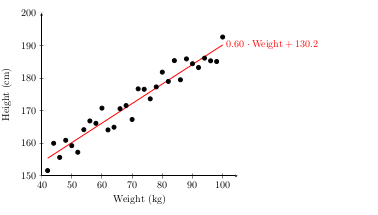
\includegraphics[width=\columnwidth,height=0.1\textheight]{linear}
%  %\caption{A caption}
%\end{figure}

%---------------- Events ok but too long list
%\begingroup
%\CTFont% tables in \small size
%\CTFont[tiny]% tables in \tiny size
%\begin{figure}[t]
%{\footnotesize
%\input{/home/frederic/researchwork/MyFirstWindow/Latex/events}
%}
%\end{figure}
%\endgroup
%-------------------------------------------------------------------------

%\begin{figure}[t]
%{\footnotesize
%\input{/home/frederic/researchwork/MyFirstWindow/Latex/eventsContacts}
%}
%\end{figure}

\begin{figure}[t]
{\footnotesize
\input{/home/frederic/researchwork/MyFirstWindow/Latex/skillsCheese}
\scalebox{.75}{\input{/home/frederic/researchwork/MyFirstWindow/Latex/contactsCheese}}
}
\end{figure}

\begin{figure}[t]
{\footnotesize
\input{/home/frederic/researchwork/MyFirstWindow/Latex/skillsGraph}
}
\end{figure}

%\begin{figure}[t]
%{\footnotesize
%\input{/home/frederic/researchwork/MyFirstWindow/Latex/contactsCheese}
%}
%\end{figure}

\begin{figure}[t]
{\footnotesize
\input{/home/frederic/researchwork/MyFirstWindow/Latex/contactsGraph}
}
\end{figure}

%\begin{figure}[t]
%{\footnotesize
%\input{/home/frederic/researchwork/MyFirstWindow/Latex/tasks}
%}
%\end{figure}

\begin{figure}[t]
  \centering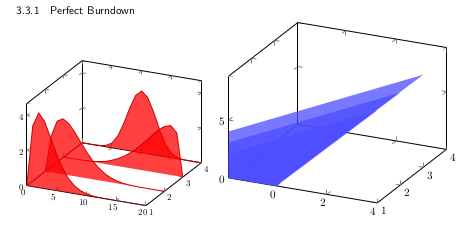
\includegraphics[width=\columnwidth,height=0.1\textheight]{burndown}
\end{figure}

%\begin{figure}[t]
%{\footnotesize
%\input{/home/frederic/researchwork/MyFirstWindow/Latex/tasks}
%}
%\end{figure}

\begin{figure}[t]
  \centering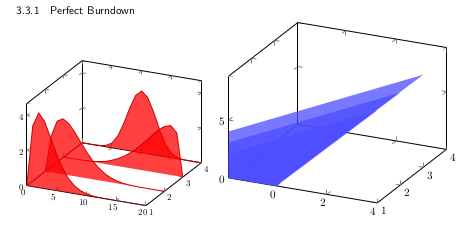
\includegraphics[width=\columnwidth,height=0.1\textheight]{burndown}
\end{figure}

%\begin{figure}[t]
%  \centering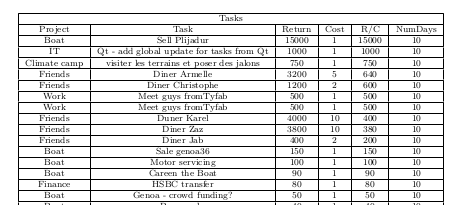
\includegraphics[width=\columnwidth,height=0.1\textheight]{/home/frederic/researchwork/MyFirstWindow/Latex/tasks}
%  \caption{A caption}
%\end{figure}

% Ici on change pour ne mettre les éléments que sur une seule colonne, c'est à dire la page complète
\begingroup
\onecolumn
\begin{figure}[t]
  \centering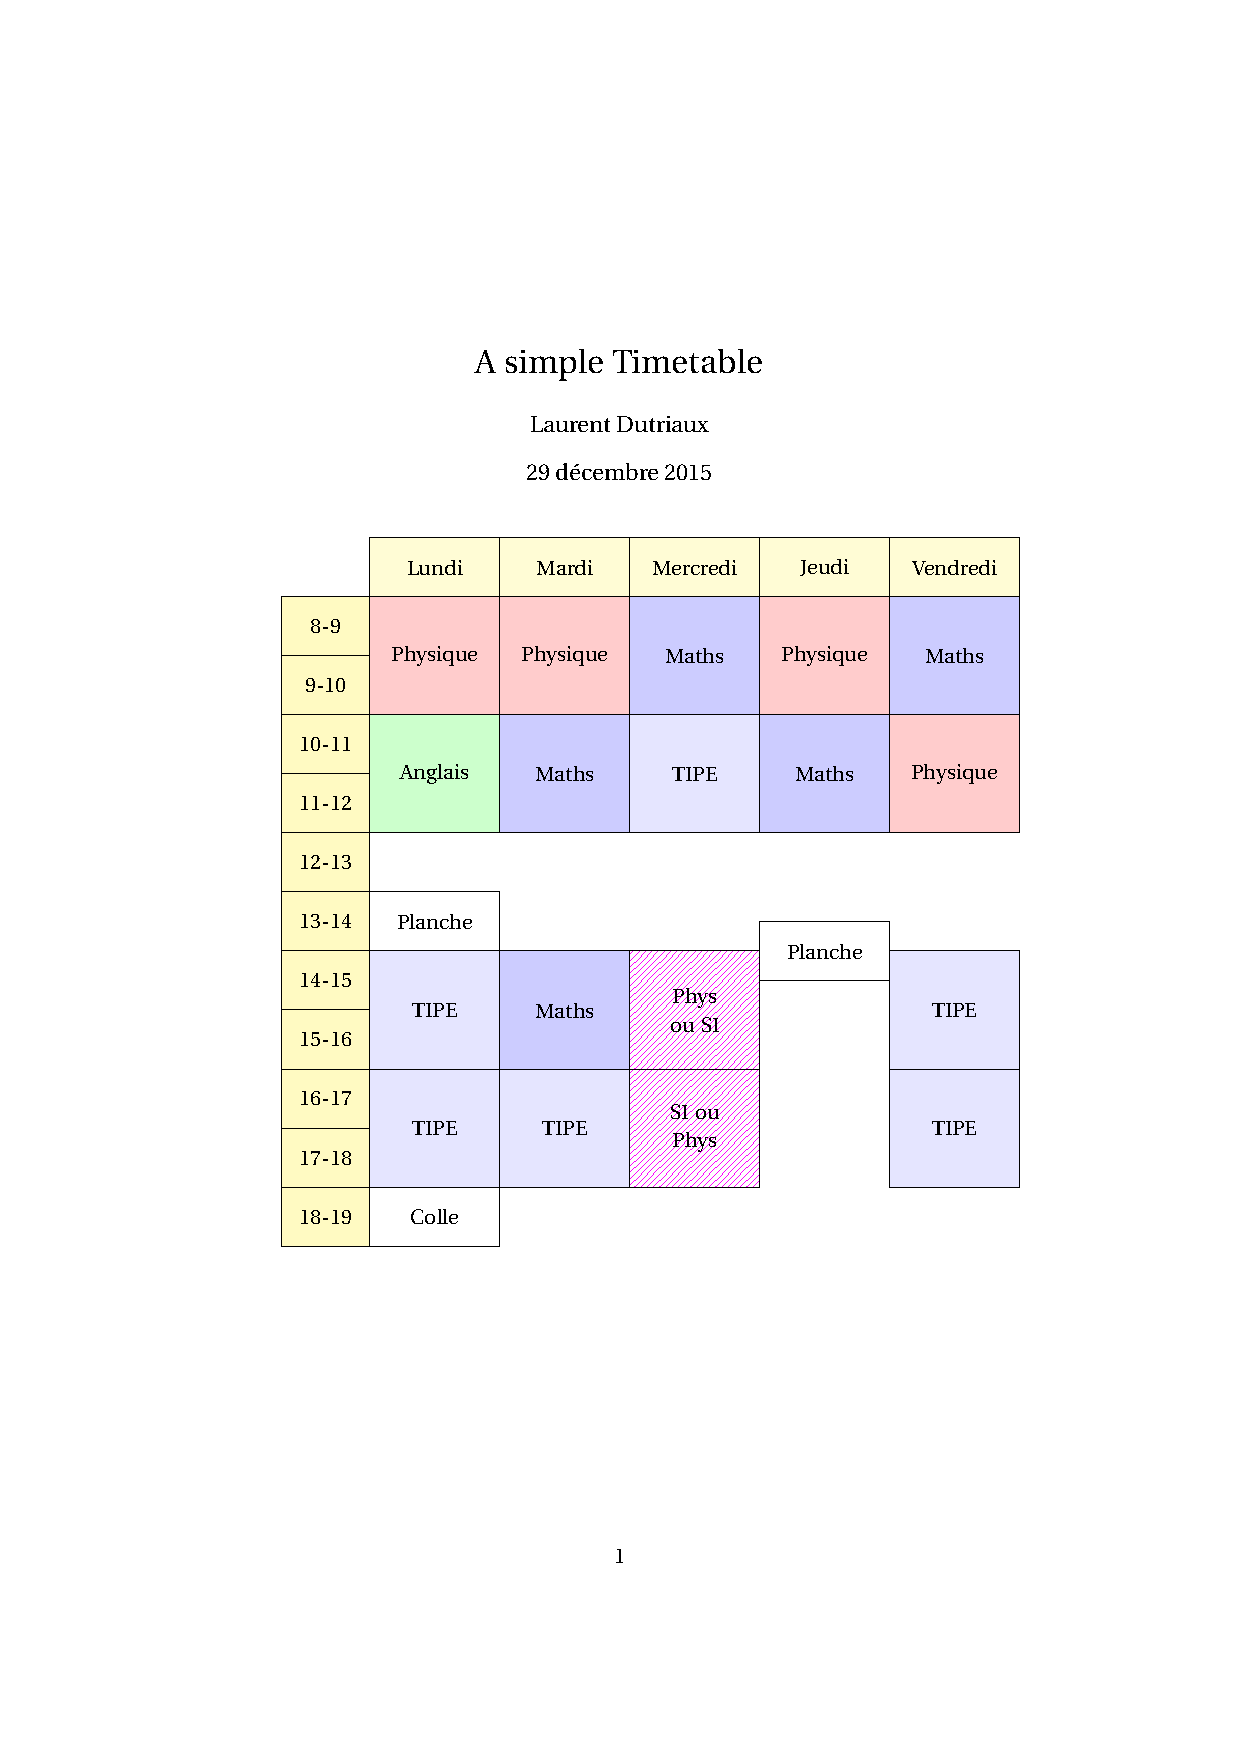
\includegraphics[width=\columnwidth,height=1.0\textheight]{TimeTable}
  \caption{A caption}
\end{figure}
\endgroup

\end{document}
